\subsection{Localisation}
\label{subsec:models/kf/localisation}
We introduce the map vector $\vec M$ which contains position and feature vectors of landmarks in our environment.
\begin{align}
	\vec M = 
		\begin{bmatrix}
			\vec m_1 \\
			\vdots \\
			\vec m_K
		\end{bmatrix}
\end{align}
where $\vec m_k$ contains the location and features of the $k^{\text{th}}$ landmark, $\vec m_k \in \mathbb R^d$ and $\vec M \in \mathbb R^{Kd}$. In the localisation problem, we assume $\vec M$ is known and so the graphical model looks as follows:
\begin{figure}[!htb]
\centering
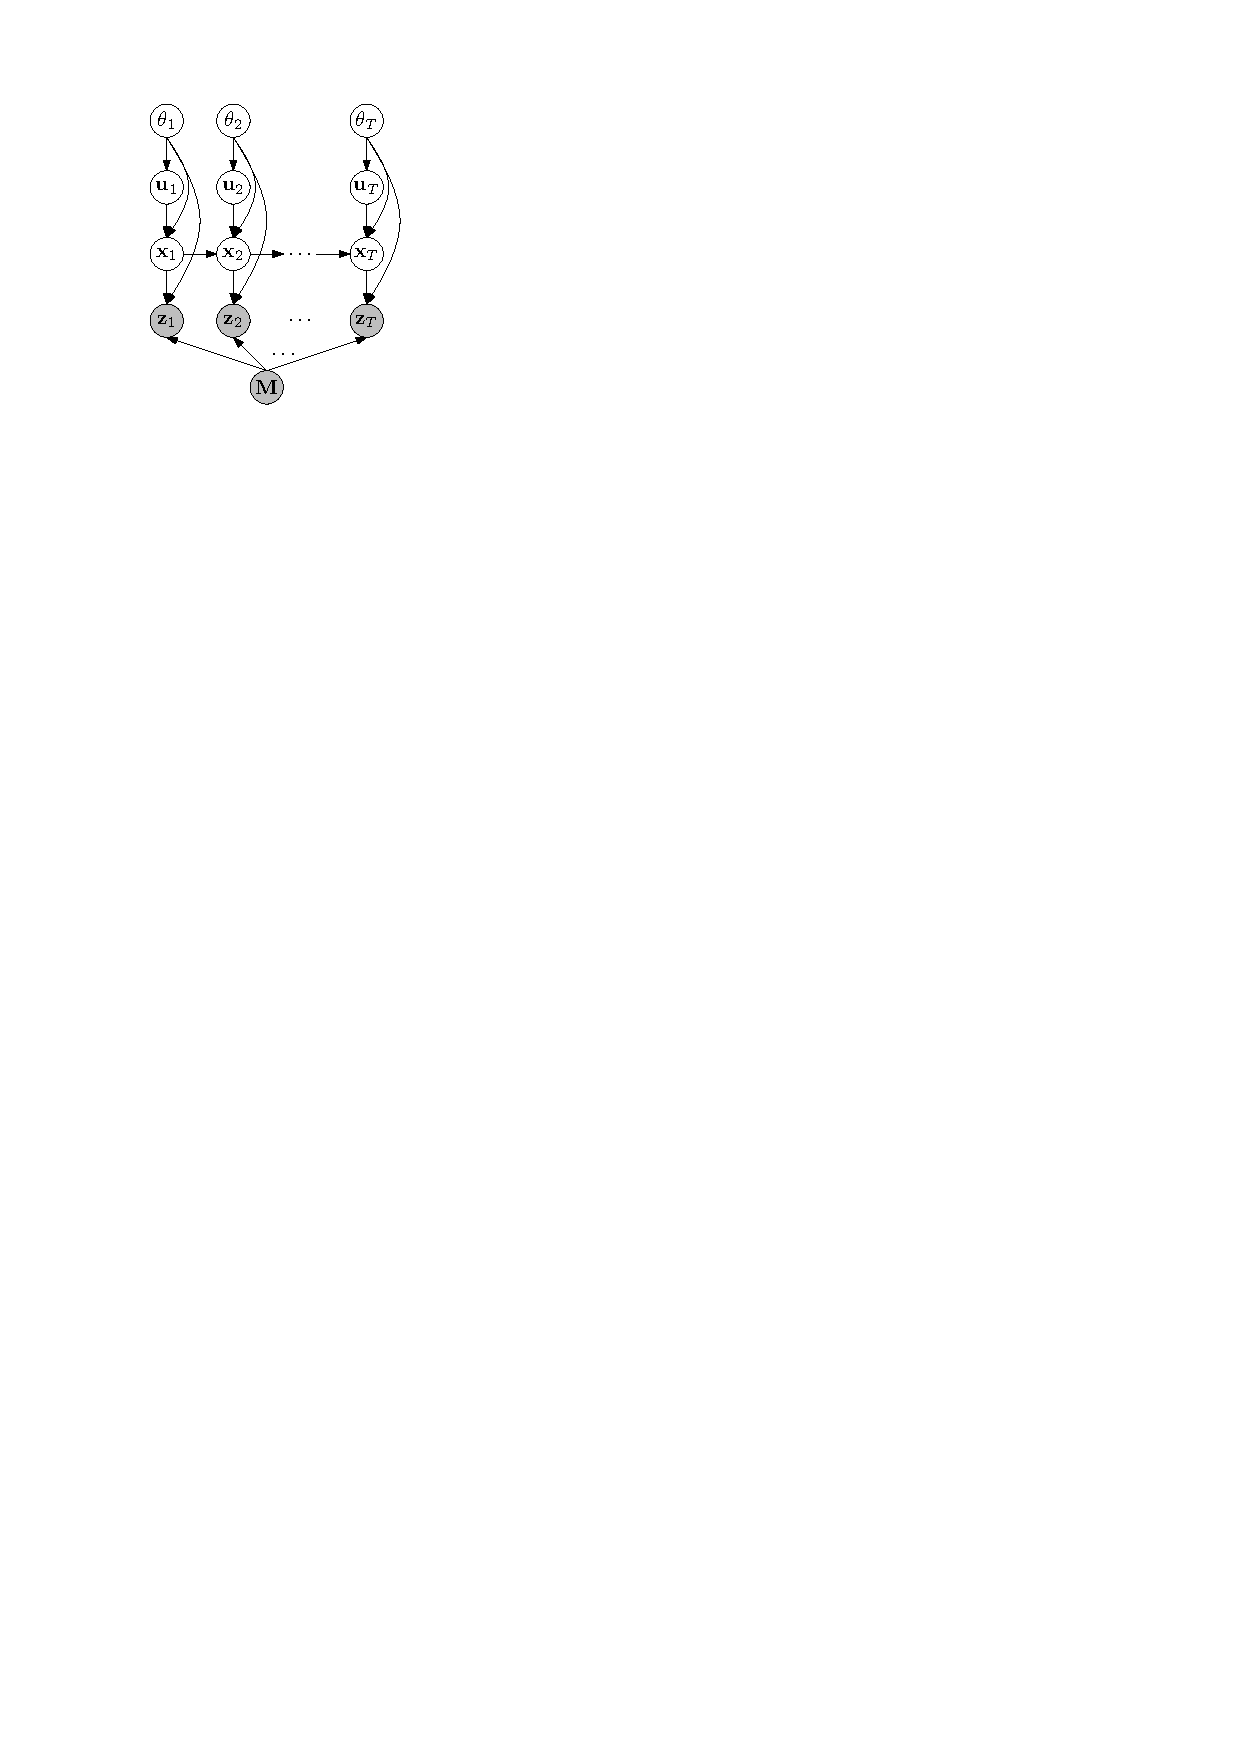
\includegraphics[scale=1]{models/kf/figures/kf-loc}
\caption{Probabilistic Graphical Model for the Kalman Filter for Localisation.}
\label{fig:models/kf/figures/kf-loc}
\end{figure}

The model can be described, for $t = 1, \dotsc, T$, by the following equations:
\begin{align}
	\vec x_t 			&= \vec g(\vec x_{t - 1}, \vec u_t) + \vec \epsilon_t \\
	\vec z_t 			&= \vec h(\vec x_t, \vec u_t, \vec M) + \vec \delta_t \\
	\vec \epsilon_t 	&\sim \Gauss(\vec 0, \vec Q_t) \\
	\vec \delta_t		&\sim \Gauss(\vec 0, \vec R_t)
\end{align}

This model almost exactly resembles the Extended Kalman filter. The update and prediction equations only differ in that
$\vec G_t \triangleq \frac{\partial \vec g(\vec x, \vec u, \vec M)}{\partial \vec x}$ instead of $\vec G_t \triangleq \frac{\partial \vec g(\vec x, \vec u)}{\partial \vec x}$. These expressions are evaluated at $\vec x = \vec \mu_{t - 1 \mid t - 1}$ and $\vec x = \vec \mu_{t \mid t - 1}$ in the case of prediction and update equations respectively.